% EMPR 2014/2015 Project report for hand in Week 3 Summer 2015

\documentclass[a4paper, 11pt]{report}
\usepackage[utf8]{inputenc}
\usepackage[pdftex]{graphicx}
\usepackage[margin=1.2in]{geometry}
\newcommand{\HRule}{\rule{\linewidth}{0.5mm}}
\usepackage{fancyhdr}
\setlength{\headheight}{15.2pt}
\pagestyle{fancyplain}
\fancyhead[LE,RO]{}
\fancyfoot[LE,RO]{\thepage}
\fancyfoot[LO,CE]{Chapter \thechapter}
\fancyfoot[CO,RE]{Douglas Parsons}


% Rewritten the Chapter settings, in order to remove the stupid 50Space 
% Indent from the top of the page. 
\makeatletter
\def\@makechapterhead#1{%
    \vspace*{10\p@}% %%% removed!
    {\parindent \z@ \raggedright \normalfont
        \ifnum \c@secnumdepth >\m@ne
        \huge\bfseries \@chapapp\space \thechapter
        \par\nobreak
        \vskip 20\p@
        \fi
        \interlinepenalty\@M
        \Huge \bfseries #1\par\nobreak
        \vskip 40\p@
}}
\def\@makeschapterhead#1{%
    \vspace*{10\p@}%
    %%% removed!
    {\parindent \z@ \raggedright
        \normalfont
        \interlinepenalty\@M
        \Huge \bfseries  #1\par\nobreak
        \vskip 40\p@
}}
\makeatother

\begin{document}
\begin{titlepage}
\begin{center}

% Upper part of the page. The '~' is needed because \\
% only works if a paragraph has started.

\includegraphics[width=0.15\textwidth]{./logo}~\\[1cm]

\textsc{\LARGE University of York}\\[1.5cm]

\textsc{\Large Second Year Project}\\[0.5cm]

% Title
\HRule \\[0.4cm]
{ \huge \bfseries Embedded Systems Project Written Report \\[0.4cm] }

\HRule \\[1.5cm]

% Author and supervisor
\noindent
\begin{minipage}[t]{0.4\textwidth}
\begin{flushleft} \large
\emph{Author:}\\
Douglas \textsc{Parsons}
\end{flushleft}
\end{minipage}%
\begin{minipage}[t]{0.4\textwidth}
\begin{flushright} \large
\emph{Supervisor:} \\
Dr.~M.J. \textsc{Freeman}
\end{flushright}
\end{minipage}

\vfill

% Bottom of the page
{\large \today}

\end{center}
\end{titlepage}

\tableofcontents
\chapter{Introduction}
% Guidance - 2 pages
% A summary of your project work, experiences as a team, expectations and
% actual outcomes, and some 'feel' for what the rest of your report is about
\section{Summary of project work}

\section{Experiences as a team}
\section{Expectations and actual outcomes}
\section{What is in the report}
This report sets out to provide a description of our team solution to the set 
assignment, as well as highlighting areas of individual contribution throughout.
The report will begin with a technical description of the set problem, 
including a discussion of requirements and technical challenges that may be 
faced in the meeting of these requirements. 
Following a description of the problem, the group solution will be discussed. 
The discussion will highlight how each section of the requirements has been met 
by the implemented solution, as well as detailing how the problem has been broken 
down for each individual member, presenting each members implementation and 
technical innovation. 
After a discussion of the group's solution, the appropriate testing strategies 
and methods that were used throughout the project will be examined in detail, 
providing feedback on how they have proved useful, and incorporating a 
discussion on a professional/social/ethical/environmental aspect of the solution.
The report will then focus critically on my individual implementation, 
detailing the technical innovation, implementation, and testing undergone for my 
contribution. 
Finally the report will conclude with a reflective summary of work 
undertaken, considering which aspects of the project went smoothly, which areas
did not go as smoothly, how this might be improved in future, and what lessons 
can be taken away from the completion of the project. 

\chapter{Technical Description of Problem}
% Guidance - 3 pages
% A technical description of the problem in terms of the requirements given,
% expanded into a discussion and highlighting likely implied technical aspects
% and challenges that need/needed to be tackled
\section{Description of Problem and Requirements}

The Embedded Systems Project consisted of two main sections: a group solution 
that was required to meet a set specification, and an individual extension to 
the group's solution that was left up to each person to determine. 
Both sections of the project involved embedded systems software development in 
the C programming language. 
\par\bigskip\noindent
The target platform of the project is an ARM-based microcontroller, 
situated on a board of peripheral accessories. 
The microcontroller consists of 
an interface board coupled with the ARM cortex-M3 based LPC1768, providing easy 
interaction via USB cable to transfer binaries, and simplifying the process of 
serial communication \cite{how-mbed-works}.
The MBED board is also sat on a board of peripheral accessories, enabling 
interaction with a variety of different components. The board is pictured below
\cite{mbed-picture}.
\begin{center}
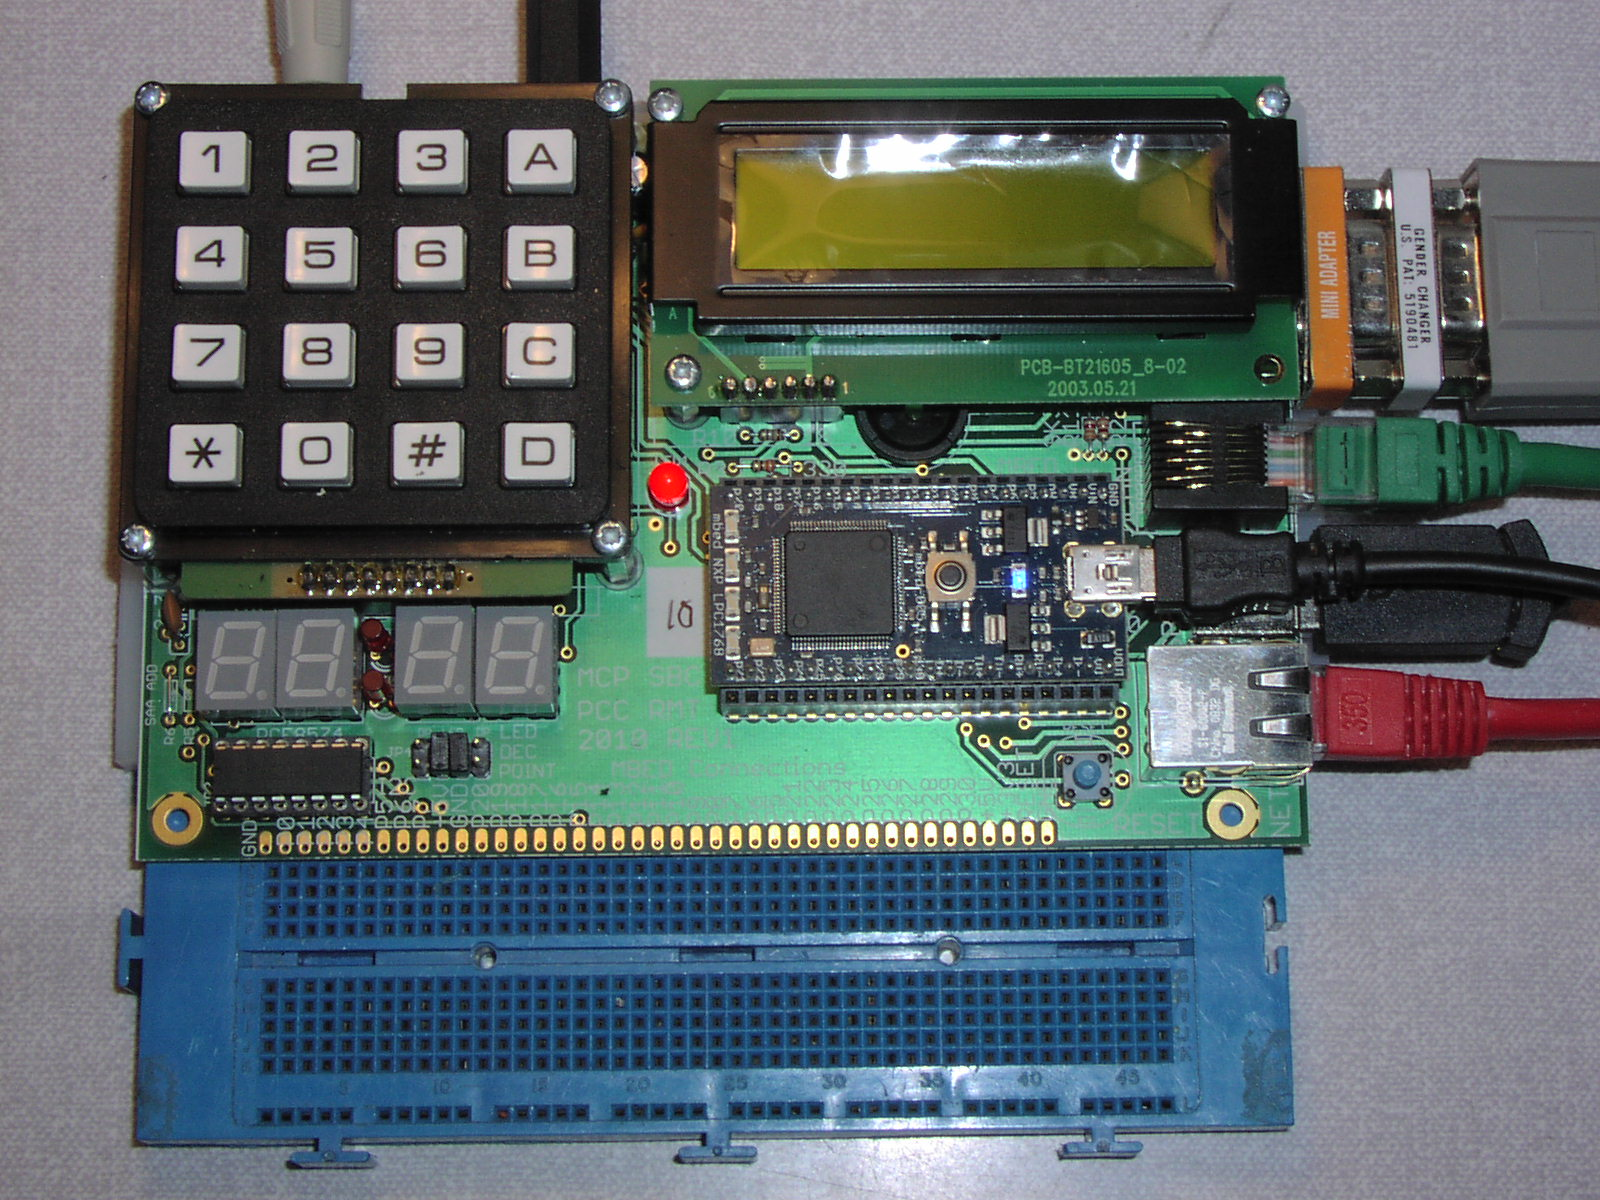
\includegraphics[width=0.80\textwidth]{./mbed_board}
\end{center}
Accessories on the board include: a 16 key keyboard, 
a 16 by 2 line LCD, four seven segment displays, a micro SD slot, a USB host 
connection, CAN bus connector, audio in and out jacks, a TCP/IP connection, as 
well as off board connections to user definable hardware. 
Interaction with these devices is achieved directly through the manipulation of 
the MBED board's pins, therefore enabling a high level of communication with 
relative ease \cite{mbed-pins}. 
The range of devices provides a large variety of possible methods for meeting 
the specification aims, and enables a large scope for individual creativity with 
extensions to the specification.
\par\bigskip\noindent
The group task consisted of multiple different challenges, with the concept
that the MBED board would continually receive CAN packets, filter out those 
that do not match a user selectable id, decode the CAN packets, and play notes 
corresponding to the frequency, volume, and duration that were specified from 
the CAN transmissions. In addition the user must be able to view useful 
information, select the channel id, and adjust the volume. The full requirements
for the group solution are as follows \cite{specification}:
\par\bigskip\noindent
\textbf{S.1. A solution using MBED for live monitoring of CAN bus data packets.}
\hangindent=0.7cm
Ideally this should include the ability to show all data and also 
to show data filtered according to a configurable instrument channel ID.
\par\bigskip\noindent
\textbf{S.2 An MBED solution which has the following specifications :-}
\begin{itemize}
        \item Receives CAN bus data continuously
        \item Has the ability to preset a local 'ID”
        \item Can optionally filter the data according to it matching the preset ID
        \item For each data element, will generate an audio tone corresponding to frequencies,
            durations, and volume levels if specified in the data stream
        \item Has a visual display on the MBED host board indicating useful information
        \item Has the ability to receive user input via keypad, or an alternative
        \item Has a volume control function
\end{itemize}
\noindent
In addition to the group solution, each individual was required to extend their 
groups implementation.  
This extension did not have to match any set specification, and was instead left 
up to each individual to decide.
For my individual extension, I implemented a shell style user interface. 
This allows user to interact with the device by typing commands into a terminal 
on their computer, effectively adding an additional element of user control that 
is both more intuitive and more responsive than using the 16 digit keypad, from 
the MBED peripherals board.
\par\bigskip\noindent
For our group solution, the specification was broken down into three separate 
areas. This allowed us to focus our expertise and interests on the aspect best 
suited to each group member.
The breakdown of the three sections was as follows: 
\begin{itemize}
    \item 
        The receiving and decoding of CAN packets (CAN bus) 
    \item 
        Generation of audio samples corresponding to frequency, duration and 
        volume (Audio)
    \item 
        User interaction with the device in order to display information 
        and adjust settings.
\end{itemize}

\section{Discussion of Technical Aspects and Challenges}

As previously mentioned, my group deconstructed the specification into three 
main areas of technical challenge. The first of these challenging areas regarded 
the receiving of data from the CAN bus, and the decoding of the packets received
to extract their content. As the CAN packets are not arriving at regularly 
timed intervals, the solution to this problem is required to be interrupt based. 
However, due to the nature of the CAN packets, a very large number can arrive in 
a comparatively short space of time. This therefore requires a highly optimised 
solution, in order to prevent packets either being missed, or race conditions 
within the interrupt handler from occurring. 
\par\bigskip\noindent
The second technical challenge of the project is the generation of audio tones 
corresponding to frequency, duration and volume levels as specified by the CAN 
packets. The CAN packets do not contain information detailing what each note 
should sound like. As a result, all musical notes need to be generated from 
first principals, for example using a look up table detailing values for a note 
at each moment in time. In combination, to make the notes sound more realistic, 
each note must go through at least three stages. The first of these stages 
defines the initial playing of a note, plucking a string or pressing a key. This
 is known as 'attack'. The second stage corresponds to the continual noise made 
from the note until it is stopped and is known as 'sustain'. The final stage 
details the note as it dies down and stops and is known as 'release'. This 
presents additional problems as each note requires multiple states, and needs to 
be tracked in its progress through each. 
Furthermore, it may be an additional desire to play more than one note at any 
one moment in time. This requires synthesis of multiple different notes in order 
to produce an appropriate output. The mathematics of this can be expensive to 
compute, and furthermore, an increase in the number of notes can drastically 
increase the processing time. A delay in the output of the notes can lead to 
a strange sounding finished product, so the efficiency of any synthesis 
calculations are paramount to the end product. 
\par\bigskip\noindent
The third technical challenge that can be presented is the user's control over 
the device. The specification determines that the user must be able to control 
the volume of the output, alter which channel of notes is being played, 
and view useful information on the MBED board. This requires a level of
interaction, most likely via the 16 digit keypad on the device, however this 
could be via alternate input methods, such as a computer keyboard. The user's 
interaction with either device once again may not be continual, but may either 
be polled, at the cost of system resources, or interrupt based. Further 
challenges are presented as any possible user input must be stored on the device, 
parsed on command, and then the desired command must be executed without any 
significant effect on the audio output. Furthermore, the challenge is made 
increasingly difficult by the required ability to interface with the entire 
project: the audio synthesis code and the CAN bus code must be fully understood 
in order to be manipulated through the user's input. 

\chapter{Description and Discussion of Team-based Solution}
% Guidance - 4 pages
% Description and discussion of the TEAM solution, noting how the team broke
% down the problem for team members and detailing the technical innovation and
% implementation of the work.
\section{Description of the Team Solution}

The team solution following the completion of the project was a successful 
working product. Every point on the specification was fully met, and the solution 
incorporated additional features such as a user friendly shell style input, or 
the ability to synthesise multiple channels of music. This chapter sets out a 
full technical description of each different aspect of the finished product, 
explaining in detail how each feature is implemented. 

\subsection*{Controller Area Network Bus Processing}

The first technical challenge faced in the implementation of the group's solution
was the retrieval of data from the controller area network bus (CAN bus). The 
implemented solution uses an advanced system to ensure that no transmissions of 
data packets are missed. 
Each time data is transmitted on the CAN bus the MBED board receives an interrupt. 
The interrupt service routine copies the data transmitted on the CAN bus into 
the devices memory, ready for processing at a later stage. 
By avoiding the processing of any data in the interrupt handler, it is ensured 
that no race conditions can occur, and therefore data transmissions cannot be 
missed. 
\par\bigskip\noindent
The data packets are stored in memory as a queue. 
This enables a first-in-first-out approach to processing of the data to occur. 
The CAN data packets are decoded according to the given specification. 
There are two possible types of packets received: A basic data packet containing 
information for the frequency, volume, channel and control data of a note, or, 
a text packet, containing information for a track name, beats per minute of the 
track, and channel numbers and names \cite{data-packet}.
If the packet received is a data packet, it interacts directly with the audio 
code, turning on, off, or adjusting notes corresponding to the information 
contained. 
Alternatively, if the packet is a text packet, it requires further processing to 
extract the information contained. 
\par\bigskip\noindent
Text packets may arrive in multiple packets due to the length of text contained. 
Following the arrival of text packets, a check-sum is sent. 
If the length of the text received does not match the value of the check-sum, 
the text is ignored. 
This ensures all packets were successfully received, and that no packets have 
been corrupted. 
If the check-sum value is correct, and the text packets have been correctly 
received, they are parsed in order to extract their content into a more usable 
format. 
This is achieved through a state based text-parser, that draws inspiration from 
a stack-overflow post \cite{text-parser}. 
The text parser iterates through the text, alternating state depending on whether 
the current location is within a word, inside quotation marks or inside 
white-space. 
This breaks the text into smaller sections and removes quotation marks, 
enabling it to be presented in a useful format, such as displaying the track 
name on the LCD display, or on the computer screen. 

\subsection*{Shell User Interface}

To provide a user friendly and simplistic user interface, enabling a high level 
of control and interaction with the device, a shell style user interface was 
created. 
Typically used for interaction with a computer, a shell is a device that takes 
a user input, and converts their input (command) into the desired functionality. 
Simply put, a shell is "a program that takes your commands from the keyboard and 
gives them to the operating system to perform" \cite{shell-def}.
For the MBED system, communication with the device occurs via serial, with a 
computer running GNU screen (terminal) used for both input, and feedback from 
the device. 
This enables the user to enter commands via the computer keyboard, or other input
method, and the MBED device to then execute these commands. 
\par\bigskip\noindent
When a character is entered into the computer terminal, an interrupt is generated
on the host MBED board. 
The interrupt handler first determines whether the user's input is a special case 
character (BACKSPACE, or ENTER), or a regular character. 
If the input is a regular character, it is stored in memory for processing at a 
later stage, as well as being transmitted over serial to be displayed on the 
computer screen. 
If the input character is BACKSPACE the last character is removed from the 
stored input, and a special character sequence is sent to the computer in order 
to delete the displayed characters from the screen. This only occurs if the 
user has an input to delete 
Finally, if the user inputs the ENTER key, a flag is toggled on, indicating that 
the user's input requires processing. Processing of the user's input is not done 
in the interrupt handler in order to avoid unpredictable behaviour through race 
conditions.  
\par\bigskip\noindent
Processing of the user's input occurs in three different stages. 
First the input is parsed, where it is split up into separate words. This 
simplifies the logic needed to determine the correct functionality to perform.
Parsing is done using a similar method as the CAN bus text packets \cite{text-parser}, 
however, modifications have been made to set a limit on the word count of the 
user's input. This prevents the situation where an input consisting of a large 
number of separate words results in excessive memory consumption, causing the 
device to crash. 
Following the parsing of text, the user's input is matched to possible input 
commands using strcmp for string comparisons. This determines the correct 
functionality of the user's input. 
Once the correct functionality has been determined, the user's command is executed. 
Depending on what this command is, interaction may involve alterations being made 
to variables, states of the system, or may interface with the audio, or CAN bus 
segments of the group solution. 

\subsection*{Keypad and LCD interaction}

The keypad and the LCD additionally provide useful tools for interaction with 
the device. The specification states that the user must be able to display 
useful information on the host board, explicating the need to incorporate the 
LCD display into the solution \cite{specification}. 
The keypad was configured to work on an interrupt based system, as opposed to 
a poll-based system. This generated an interrupt each time a key was pressed. 
The interrupt handler first determined whether the user input was a valid key, 
filtering out any undesired interrupts generated from the row and column 
scanning of the keypad. 
Furthermore, a debounce system was generated, only allowing one successful 
interrupt to occur once every half a second. This was incorporated using SysTick
to determine the difference in time between inputs. 
Following a successful input, the correct functionality was then determined and 
executed, 
\par\bigskip\noindent
The LCD display was heavily utilised by the group solution, and had a wealth of 
features. 
The LCD code enabled writing to only a section of the display, allowing different 
information to be displayed on each line. 
This was achieved by manipulation of the device drivers, writing to only a 
section of the displays memory prior to updating the display. 
Furthermore the LCD display was further extended, adding the capability for 
scrolling text. 
This was implemented using pointer manipulation to incrementally iterate through 
a text string, and periodically update the display with this string using 
a system timer (SysTick).  

\subsection*{Audio Processing}

The audio processing aspect of the group solution was very thorough, and 
incorporated a vast array of different features to produce a high quality of 
sound from the end product.
\par\bigskip\noindent
No information is known about the audio output, and wave-forms must be generated 
from first principles. This is implemented using a look-up table, 

\section{How the problem was broken down for individual members}

The breakdown of our solution into components individual members could work on 
was a great strength of our team. Each person worked on an aspect of the project 
that they found interesting, and throughout the project we had regular feedback 
on all our work in order to make sure we were meeting our specifications and 
that nobody was out of their depth. Below I have divided up the work that each 
individual completed during the duration of the project, and why they were 
working on that aspect of the project. 

\subsection*{Mingzhao Zhao}
Each individual was allowed to choose their own area of the project to work on. 
Mingzhao was not especially confident with the platform, and therefore he 
decided to target user interaction with the device via the keypad. This 
provided a possible method of user input, as well as providing a means to 
optionally filter data, or control the volume output of the device. 
Following suggestions 
of other group members he decided to convert the previous keypad polling method 
incorporated in the mini-projects into an interrupt based system, removing the 
need for unnecessary CPU cycles to be used polling the device continually. 

\subsection*{Shivam Mistry} 
Shivam worked very strongly as a group member. To begin with he took on the 
challenge of constructing code to read the data from the CAN bus continually, 
as well as implementing the base for filtering out data according to a preset ID
. Following the construction of the CAN bus code, he worked on optimising the 
CAN bus code through the
implementation of a queue, as well as decoding the CAN packets to extract their
data, and the parsing of text packets to extract only the useful information. 
Furthermore, on realisation of additional device memory, Shivam wrote a memory 
allocator allowing the additional memory to be used constructively, further 
optimising the system. 

\subsection*{Myself (Douglas Parsons)}
Following the mini projects, and from reviewing the specification, it was clear 
that a strong level of user interaction with the device would provide valuable 
debugging tools, could potentially allow settings to be changed without 
re-installing binaries on the device, and could be used for a wide range of 
useful functions, such as changing the volume or displaying song information. 
From the mini projects it became clear that the 16 digit keypad attached to the 
MBED would not provide an intuitive user experience. Rather than relying on 
the keypad as the sole method of user interaction, I instead focused 
on allowing a further degree of interaction via the computer keypad. This 
enabled the user to preset an ID to filter out data, adjust the volume of the 
output, display any data received on the CAN bus, as 
well as adjust settings within the project without requiring a full reinstate.
During the implementation of the shell it became clear that this could be a 
valuable tool for displaying useful information such as the song name, and 
therefore I additionally worked with the LCD display to enable a much greater 
degree of control over what was displayed, enabling scrolling text, and writing 
to each line of the display individually.

\subsection*{Liam Fraser}
Liam has a strong background in music technology, taking the subject at A-level,
and working on personal projects involving music. Furthermore his interest from 
the beginning of the project in audio processing meant that it was an obvious 
choice for Liam to look into the generation and playback of music. The 
specification was exceeded with his contributions, not only did his solution 
generate an audio tone corresponding to the frequency, duration, and volume 
levels specified in the data stream, but implemented an attack sustain release 
curve to improve the realism of the output sound, as well as additive synthesis 
enabling multiple notes to be played simultaneously, and his solution also 
used DMA and a fixed point library to improve the efficiency of the system. 

\section{Technical innovation and implementation of each member}
\subsection*{Mingzhao Zhao}
Mingzhao's work was primarily focused on implementing interaction via 
the 16 digit keypad on the MBED board. The keypad was set up in the mini-projects 
to allow user interaction through continually polling the keypad. However, due 
to the limited speed of the processor it was decided that a better solution 
would be to use an interrupt based system.
However, this caused additional problems with bounce on the switches: 
multiple interrupts could occur in a very short space of time due to bounces on 
the switches. Many of these interrupts generated were redundant, or gave 
nonsensical input values, and furthermore their rapidity caused race conditions 
to occur within the interrupt handler. 
Due to the row/column method in which the key pad is scanned, the 
number of bounces was reduced significantly by filtering out any inputs that 
did not match one of the keys pressed. The switch bounces were then reduced 
further by only allowing a single key press every half a second. 
This method of debounce was implemented using a system 
timer (SysTick) to count the time between successive key presses. Any key 
presses that occurred too closely together were disregarded. 

\subsection*{Shivam Mistry}
Shivam initially targeted the CAN bus, and was able to rapidly achieve a fully 
functioning prototype. The original solution processed each packet as it was 
received. However, as the complexity of songs increased it became clear that this 
simplistic method was not going to be sufficient when many CAN packets require 
processing in a short space of time.
In order to improve the functionality, a queue was implemented. Packets were 
added to the queue on being received, and processed whenever there was sufficient
processor resources available.
This removed the requirement of each packet being processed as it was received,
 and therefore provided a clean, efficient solution.
Shivam's contribution also included the reverse engineering and decoding of any
 CAN packets received through testing their check-sum, and parsing any received 
text.
As the check-sum method was not specified in any documentation, the first 
challenge was determining what the check-sum corresponded to. Values that did 
not match the length specified by the check-sum were not processed, and therefore 
could not have any impact on the system. Furthermore, the text packets sent prior 
to each song being played required parsing in order to extract any useful 
information. Therefore, a text parser, extracting the useful information from 
these packets to the device was implemented using a state based solution. 
\par\bigskip\noindent
Furthermore, following an 
instance where the physical memory (RAM) on the device was fully used up, Shivam 
discovered that the device contains an additional 32Kb of memory, 
typically reserved for communicating to a USB or Ethernet device. However, 
due to the reserved status of this memory, a memory allocator was required for 
it to be utilised. 
Therefore, the group solution contains a memory allocator allowing access to 
a further 32Kb of memory. This allows a much greater amount of information to be 
stored on the device. 
In addition, the look-up table used by the memory allocator was stored in the 
additional memory, making it a self containing allocator. 

\subsection*{Myself (Douglas Parsons)}

My personal contribution to the project was primarily targeted at the user 
interactions with the device. While it was initially set out that Mingzhao was 
going to work on implementing an interrupt based keypad, I decided that the 
communication via serial would potentially allow a much greater level of 
debugging, interaction, and manipulation of settings for the device. From the 
beginning of the ten week period, I focused on setting up a shell style interface 
for the device. This would allow the user to communicate with the MBED board by 
typing in commands on a computer keyboard, and execute the command by pressing 
the enter key. The input from the keyboard was implemented using interrupts in 
order to avoid unnecessary computation time from continual polling. 
Furthermore, the processing of text input required a text-parser to be used. 
Due to an unknown number of words, and an unknown input length, the parser had 
to be very carefully adjusted to avoid memory overflow situations. Further 
difficulty was added to the implementation, as alterations had to be made in many 
different aspects of the group solution. A detailed understanding of each 
individuals contributions was required to manipulate their functionality, and 
continual additions and updates were needed throughout the project as changes 
were made. 
In addition to implementing the additional interfacing method of a shell style 
interface, I focused on customisation of the mini-project LCD screen code in 
order to allow a greater level of control. I implemented features such as the 
ability to write to each individual line of the LCD display, and the ability to 
scroll text across the screen. 
The latter of which was particularly difficult, not only requiring pointer 
manipulation for efficient text processing, but accessing only the required 
section of the LCD in order to avoid displaying unwanted characters provided 
a significant technical challenge. Following the implementation of the shell, and 
the LCD screen code, 
I worked alongside Mingzhao on combining his code with 
the rest of the group solution. 

\subsection*{Liam Fraser}
Liam Fraser, following an interest in music technology was eager to work on the 
audio code for the project. He implemented a simplistic system, allowing musical 
notes to be generated by scanning, and interpolating over a look up table. He then 
looked into generating synthesised music, and implemented additional synthesis 
into the project, allowing multiple notes to be playing simultaneously. However, 
on testing his synthesis code on the MBED board, it rapidly became apparent that 
the use of floating point numbers was not sufficiently quick to produce clean 
sounding audio. Therefore, a fixed point library was implemented, this allowed 
much quicker calculations to occur compared to those of floating point numbers. 
Following this optimisation of the synthesis code, the synth code was further 
optimised through the use of Direct Memory Access (DMA). This allowed the audio 
output to work independent of the central processing unit (CPU). This 
therefore speeds up the processing of any audio, as the CPU does not have to be 
involved for any sound to be output, only for the generation of audio samples 
\cite{dma-book}. In addition, to create a more realistic sounding output from the 
device, an attack sustain release state model was incorporated for each note. 
This gives an initial rise in volume as the note is turned on, and a fading out 
of the note as it is turned off, producing a volume curve more typical of an 
actual instrument \cite{asr-book}.


\chapter{Evaluation and Testing of Team-based Solution}
% Guidance - 2 pages
% Details of your team's testing strategy, and the results, including how well
% the solution met the requirements. Your evaluation should include a specific
% section relating to a professional/social/ethical/environmental aspect of
% your system solution.
\section{Description of the Team's Testing Strategy}

Throughout the duration of the project, each section of the project underwent 
significant reviews, and testing in order to ensure that it was of the highest 
quality and that it was not laden with any issues causing undesirable behaviour, 
or significant faults that may have caused the device to crash. Furthermore, once 
incorporated into the group's main solution, the implemented code underwent a 
thorough review in order to ensure that the quality of the implemented product 
was the highest possible, and free from anything that may cause issues in the 
future. In effect the product underwent many different stages of testing 
throughout its lifecycle. 

\subsection*{Individual Testing}

Prior to the inclusion within a greater completed solution, each section of the 
project underwent individual tests. In order to test each section of the project, 
a debugging library was created. The debugging library was only included in the 
binaries installed on the device if the make command included included it. This 
means, for the purposes of testing it was possible to use \texttt{make debug} 
and have debug messages containing text, or values printed out over serial. 
However, once sufficient testing was done, no 
alterations had to be made to the source code to remove these statements, and 
instead the project could be installed by calling \texttt{make}. 
This enabled statements to be added to the project, that would print out 
messages over serial.

\subsection*{Code Review}

Before each contribution was incorporated into the group's solution, it was 
first checked over by at least two other group members to ensure the quality of 
the solution was high. These checks often resulted in refactoring code to 
achieve a more streamlined end product, examples of which could include the 
simplification of logic for writing text to the LCD display through pointer 
arithmetic, or simplifying code within an interrupt handler in order to avoid 
race conditions. 

\subsection*{Integration Testing}

Following the combination of individual components into the group solution, the 
combined product was then tested thoroughly to ensure no erroneous behaviour 
could occur. This was primarily done by leaving the boards running for long 
periods of time within the labs, and listening to make sure nothing unexpected 
was occuring. In addition, each feature was continually explored in order to 
make sure everything fully functioned.  

\section{Results of Testing Strategy and How Well This Met the Requirements}


\section{Section relating to a professional/social/ethical/environmental
        aspect of our solution} % TODO - Find a proper name for this section

\chapter{Description, Discussion, Testing and Evaluation of Individual 
Component}
% Guidance - 3 pages
% Description and discussion of your individual component solution, detailing
% the technical innovation and implementation and details of your testing
% strategy, and the results. 
\section{Description of Individual Component Solution}

My individual contribution to the project consisted primarily of a shell style 
interface for the host board, allowing user interaction via a computer keyboard 
and monitor, but also consisted of the modification and extension of previously 
existing LCD screen code, to allow a much greater degree of control over the 
attched LCD display. 

The shell style interface was set up using an interrupt based system from the 
computer. This enables users to enter commands through any input method for 
the computer and process them on the device. This method also allows the user
to display useful information through the computer monitor.

There were a wide range of possible input commands available through this interface, 
with many possible options and settings being adjusted on the fly. By typing 'help' and 
pressing enter, the user could view a list of possible commands, as seen below: 

% TODO - PUT THIS INTO A TABLE LOL 
"List of available commands:\par\bigskip\noindent
playnote note volume   : plays the selected midi note\par\noindent
noteoff note           : turns off any playing notes\par\noindent
volume <vol>           : sets the output volume to 'vol'\par\noindent
showvol                : displays the current volume\par\noindent
write "text"           : writes text to the LCD screen\par\noindent
writeline "text" <linenumber> : writes text to one line of the 
LCD screen\par\noindent
listen                 : listens to music on the CAN bus\par\noindent
stoplisten             : stops listening to music on the CAN bus\par\noindent
setid <channel>        : Filters out channels that do not match 
channel number 'channel'. 
To play all, use "setid all\par\noindent
showid                 : Shows the id of the current channel\par\noindent
showtrack              : Shows the current track name on the LCD\par\noindent
showchan               : Scrolls the channels on the LCD\par\noindent
showpacket             : Prints CAN packets until a key is pressed\par\noindent
scroll \"text\" <line> : displays scrolling text on line <line> of the 
LCD screen\par\noindent
stopscroll <line>      : stops scrolling text on the screen. To stop both lines, 
enter <line> as 2 or all.\par\noindent
scrollenable <line>    : enables scrolling text on the screen.\par\noindent
shownotes              : displays all notes currently being played\par\noindent
cowsay \"text\"        : displays an ASCII cow, saying text\par\noindent
clear <line>           : clears any text that is on the lcd line <line> 
Note - you may also have to call stopscroll to fully clear\par\noindent
\par\bigskip\noindent
This therefore provides the user with a high amount of control over the devices 
output though both audio and visual elements, as well as a high level of control 
over the devices functionality. Furthermore, the interaction with 
the on board LCD display can be clearly seen through the above commands, hence 
explicating the necessity for the alterations made to LCD display code to permit 
a greater degree of control, and enable features such as scrolling text, and 
writing to only part of the LCD screen. 

\section{Discussion of Technical Innovation and Implementation}

The implementation of the shell style interface and the improvement of the LCD 
display code consists of many different technical challenges, and required many 
different technical challenges throughout. First and foremost there was the 
challenge of setting up a system to enable user input to be recognised. This is 
achieved using an interrupt based system, such that each new character entered into 
a screen set up for the board will trigger an interrupt. When the interrput is 
triggered, the character that was input is transferred to the host board and stored into 
memory for processing at a later stage. This incorporated several different technical 
challenges in the implementation, such as figuring out how to set up the interrput, and 
how to allocate memory for storing any characters input. The simplest solution for 
allocating memory was used: a set input limit is defined, and any characters that are 
input past this count are not stored in memory. Other technical challenges involved handling 
special input cases such as backspace to delete a character from memory, but only if there 
was any input to delete. 
\par\bigskip\noindent
When the enter key is pressed (\\r\\n received on the interrput), processing of the user's 
input command begins. 
First the text is split up into tokens for processing. This 
requires the use of a text parser. The text parser implemented uses a state based system,
with different states corresponding to whether it is interpreting a single word, a phrase 
(group of words encased in quotation marks), or whitespace. This breaks the user's 
command into it's constituent components, which can then be individually evaluated. 
However, it was found that memory allocation problems could occur due to the large range of 
possible tokens in the input. For example, the user could input 'a a a a a a', and this 
would be interpreted as 6 individual tokens, requiring the allocation of six blocks of 
memory. A solution to this problem was found by simply setting a limit on the number 
of tokens that can be generated by a single command. 
\par\bigskip\noindent
Following the disection of the user's input into components, a string comparison tool (strcmp)
was used to determine what the user's input was, enabling the corresponding desired 
behaviour to be executed. In order to prevent race conditions from occuring within in the 
interrupt handler, all text processing following the enter key being pressed occurs 
outside of the interrupt handler using a flag based system.
\par\bigskip\noindent
In order to successfully perform the desired functionality, settings are altered within many 
different areas of the project. The implementation of the shell therefore required a 
fully detailed understanding of how each individual component of the project functions
in order to manipulate and alter existing code. Modifications were made throughout 
the project, and included; the addition of a settable id within the CAN bus code, 
the addition of a filter in the CAN bus to ignore unwanted data 
according to the preset id, the addition of a volume control in the synth code, and a major 
overhaul of existing LCD code to allow a much greater degree of control over the display. 
\par\bigskip\noindent
The overhaul of the LCD display code provided a significant technical challenge. The initial 
desire was simply to allow scrolling text on the display, however it soon became clear that 
further alterations were required. Initially the LCD code would write to the LCD display, and 
clear it. To match what I wished to achieve, it was necessary to first figure out how to write 
only to a single line of the LCD display, without clearing the other line. This required 
accessing only certain memory adresses of the LCD display buffer in order to prevent clearing 
parts of the display. Following the successful implementation of the capability to write to 
each individual line of the LCD display, the next target was to give the ability to scroll 
text across the display, in order to effectively increase the number of characters that could be read. 


\section{Testing Strategy, and the Results}

\chapter{Summary and Conclusions}
% Guidance - 1-2 pages 
% A reflective summary of the work undertaken (both team and individual),
% including thoughts about what went well, what did not, what could have been
% improved, and lessons learned. 
\section{Reflective Summary of Team Work}

Team work was an essential part of the project, and an area where my group 
excelled. Each individual was allowed to select their own areas of the project 
to work on, and furthermore regular meetings and code review sessions both ensured 
that no individual was overwhelmed, and ensured that contributions to the 
solution were of the highest quality. 
\par\bigskip\noindent
The group solution achieved every point of the specification in an elegant 
manner, and had a wealth of additional functionality through additions to the 
project. 
Examples of these additions could include; the ability to synthesise music and 
play back multiple notes on each channel and multiple channels simultaneously, 
an improved user interaction via a shell style interface complete with the 
ability to adjust settings and change mode of operation without reinstalling the 
device, or a more realistic sounding audio playback through the use of attack-
delay-sustain-release models. 

\section{Reflective Summary of Individual Work}

My individual extension project was the implementation of a Linux style shell, 
enabling user interaction with the mbed board using a computer monitor and 
keyboard via serial communication. The addition of the shell style interface 
provided a wide range of valuable tools, and a great degree of control over the 
host board. Examples of the control given includes: 
\begin{itemize}
    \item The ability to play notes
    \item The ability to change the device volume
    \item the ability to write custom text to the LCD display 
    \item The ability to change which channel of music is being listened to
    \item The ability to view useful information, such as the track name, channel,
or what notes are currently being played
    \item The ability to view CAN packets as they are received on the CAN bus 
    \item The ability to scroll text on the LCD display 
\end{itemize}
This enabled a great degree of control over the host board, and provided 
invaluable tools throughout the course of the project. This extension project 
was initially very challenging and was an ambitious task to undertake due to the 
scale of the implementation combined with any desired features. However, the end 
result was very rewarding and one that I can be proud of. 

\section{What went well}


\section{What went poorly}


\section{What could have been improved}

Due to the nature of the project, there is a large amount of extension to the 
basic functionality that can be added. Our group solution extended the base 
implementation a long way, however, additional features were nearly implemented
that could have made a good improvement to the finished product. 
There are three examples of features that were not implemented in the final 
version of our project, but would have contributed to an overall improvement of 
the project. 
The first improvement would be the incorporation of multiple wave 
tables. 
Our group solution used sine waves to generate audio samples, however, 
there is scope for allowing any wave to be used. 
Through use of the shell it would be possible to alternate between different 
wave tables without the need to reinstall the binary on the device. This would 
allow a further degree of control over the device, and could be used to alternate
to more pleasurable sounding outputs for certain channels. 
The second potential improvement that could have been made ties in to the first, 
and is the implementation of drum samples to create a more complete sounding 
audio track. On the CAN bus sixteen channels of audio data is sent


\section{Lessons Learned}



\appendix
\chapter{Specified Documents}
% Guidance - As needed
% Evidence of project management (copies of meeting minutes), and evidence of
% preparation (copies of your Autumn formative assessment sheets)
\section{Meeting minutes}
\section{Evidence of Preparation}
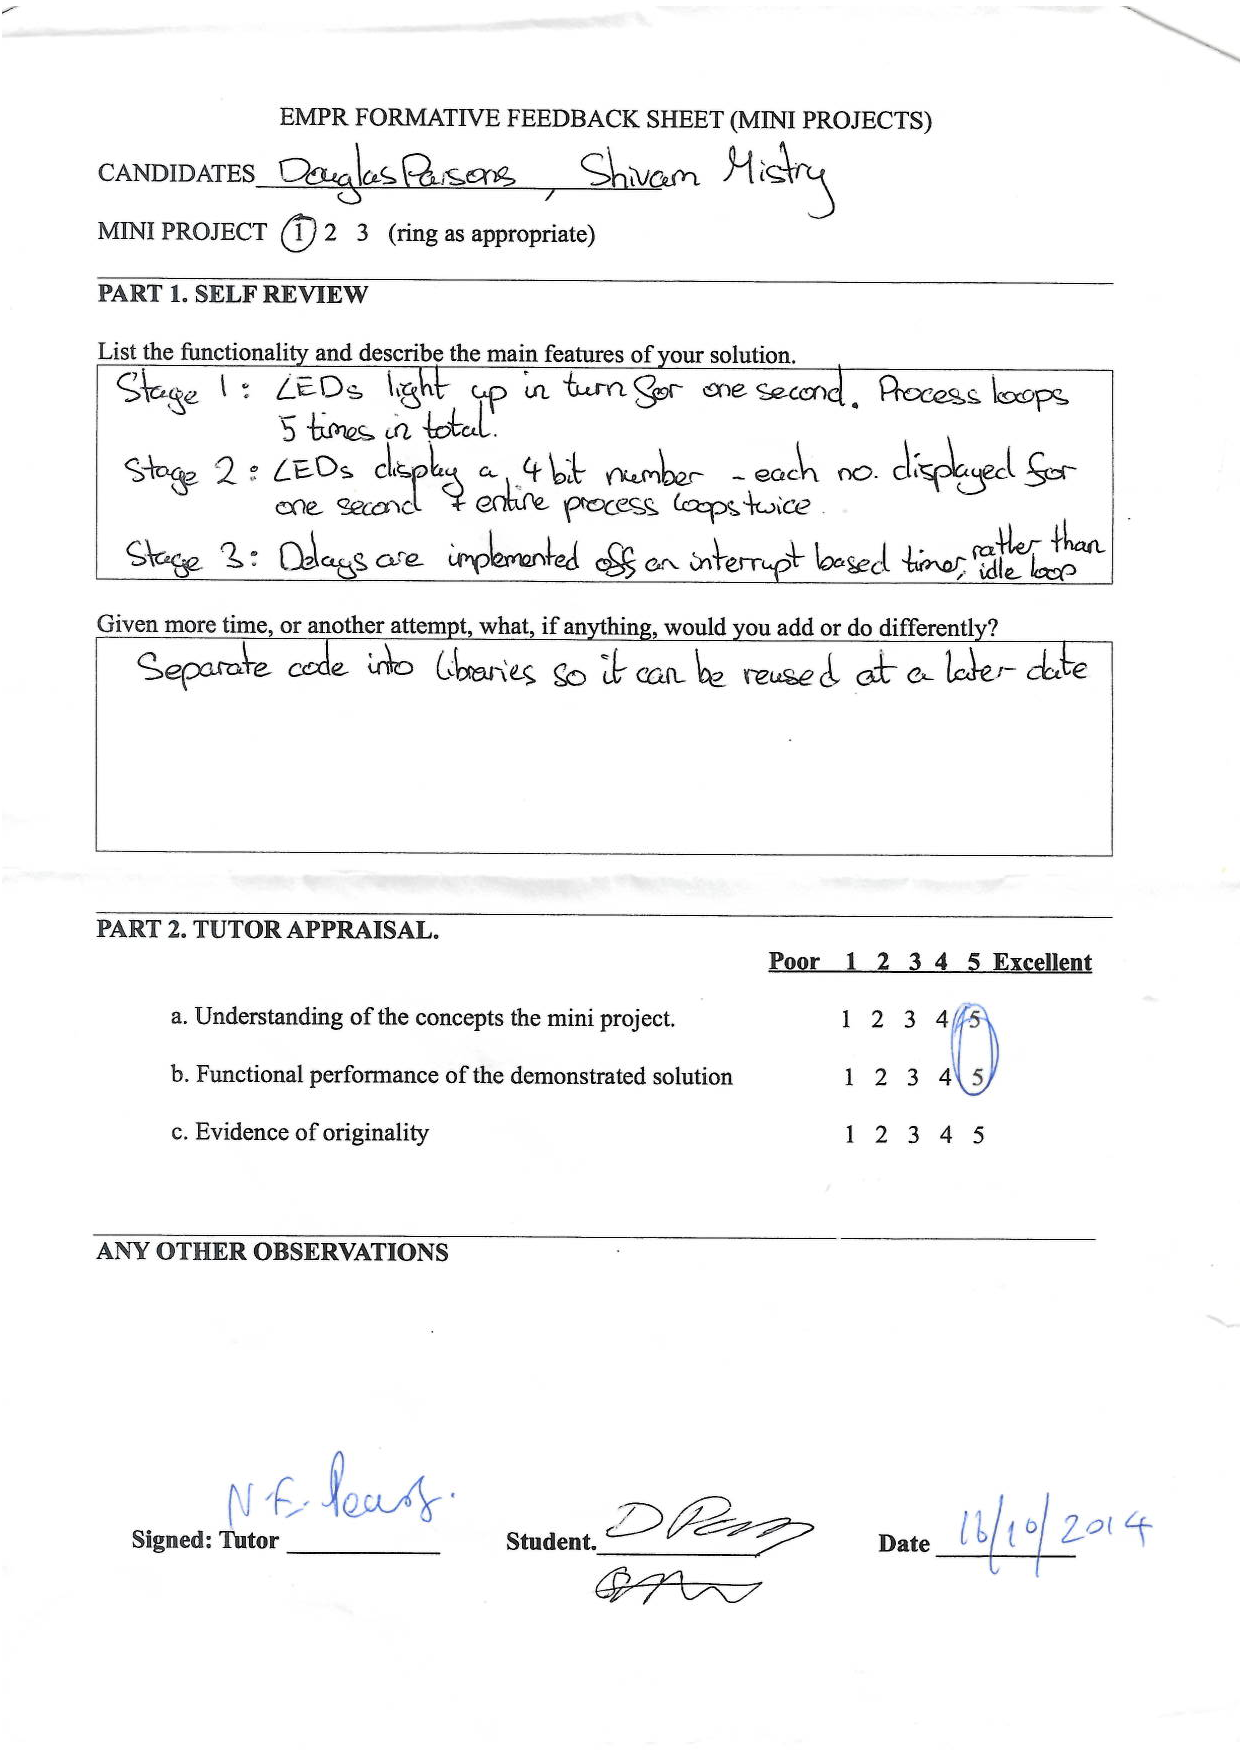
\includepdf[pages={1}]{mini_project_1.pdf}
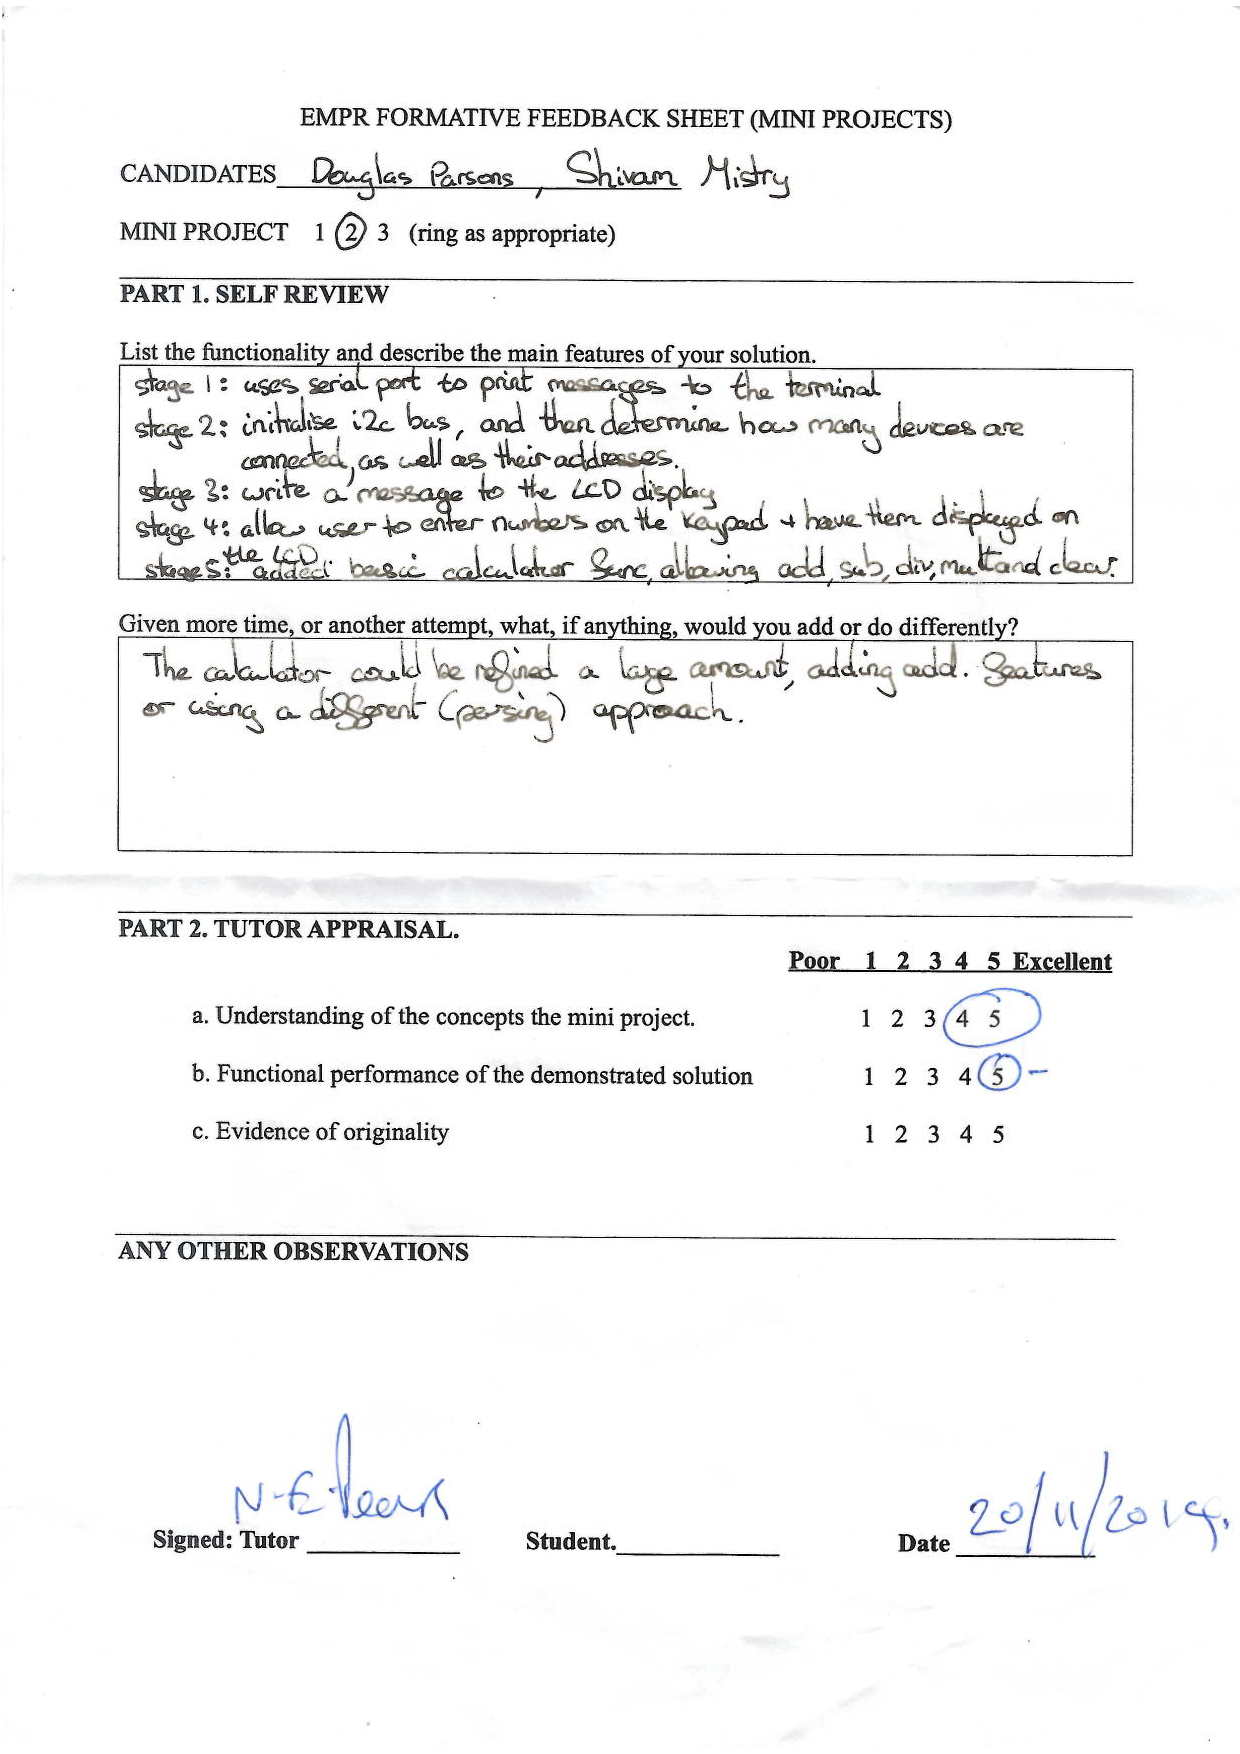
\includepdf[pages={1}]{mini_project_2.pdf}
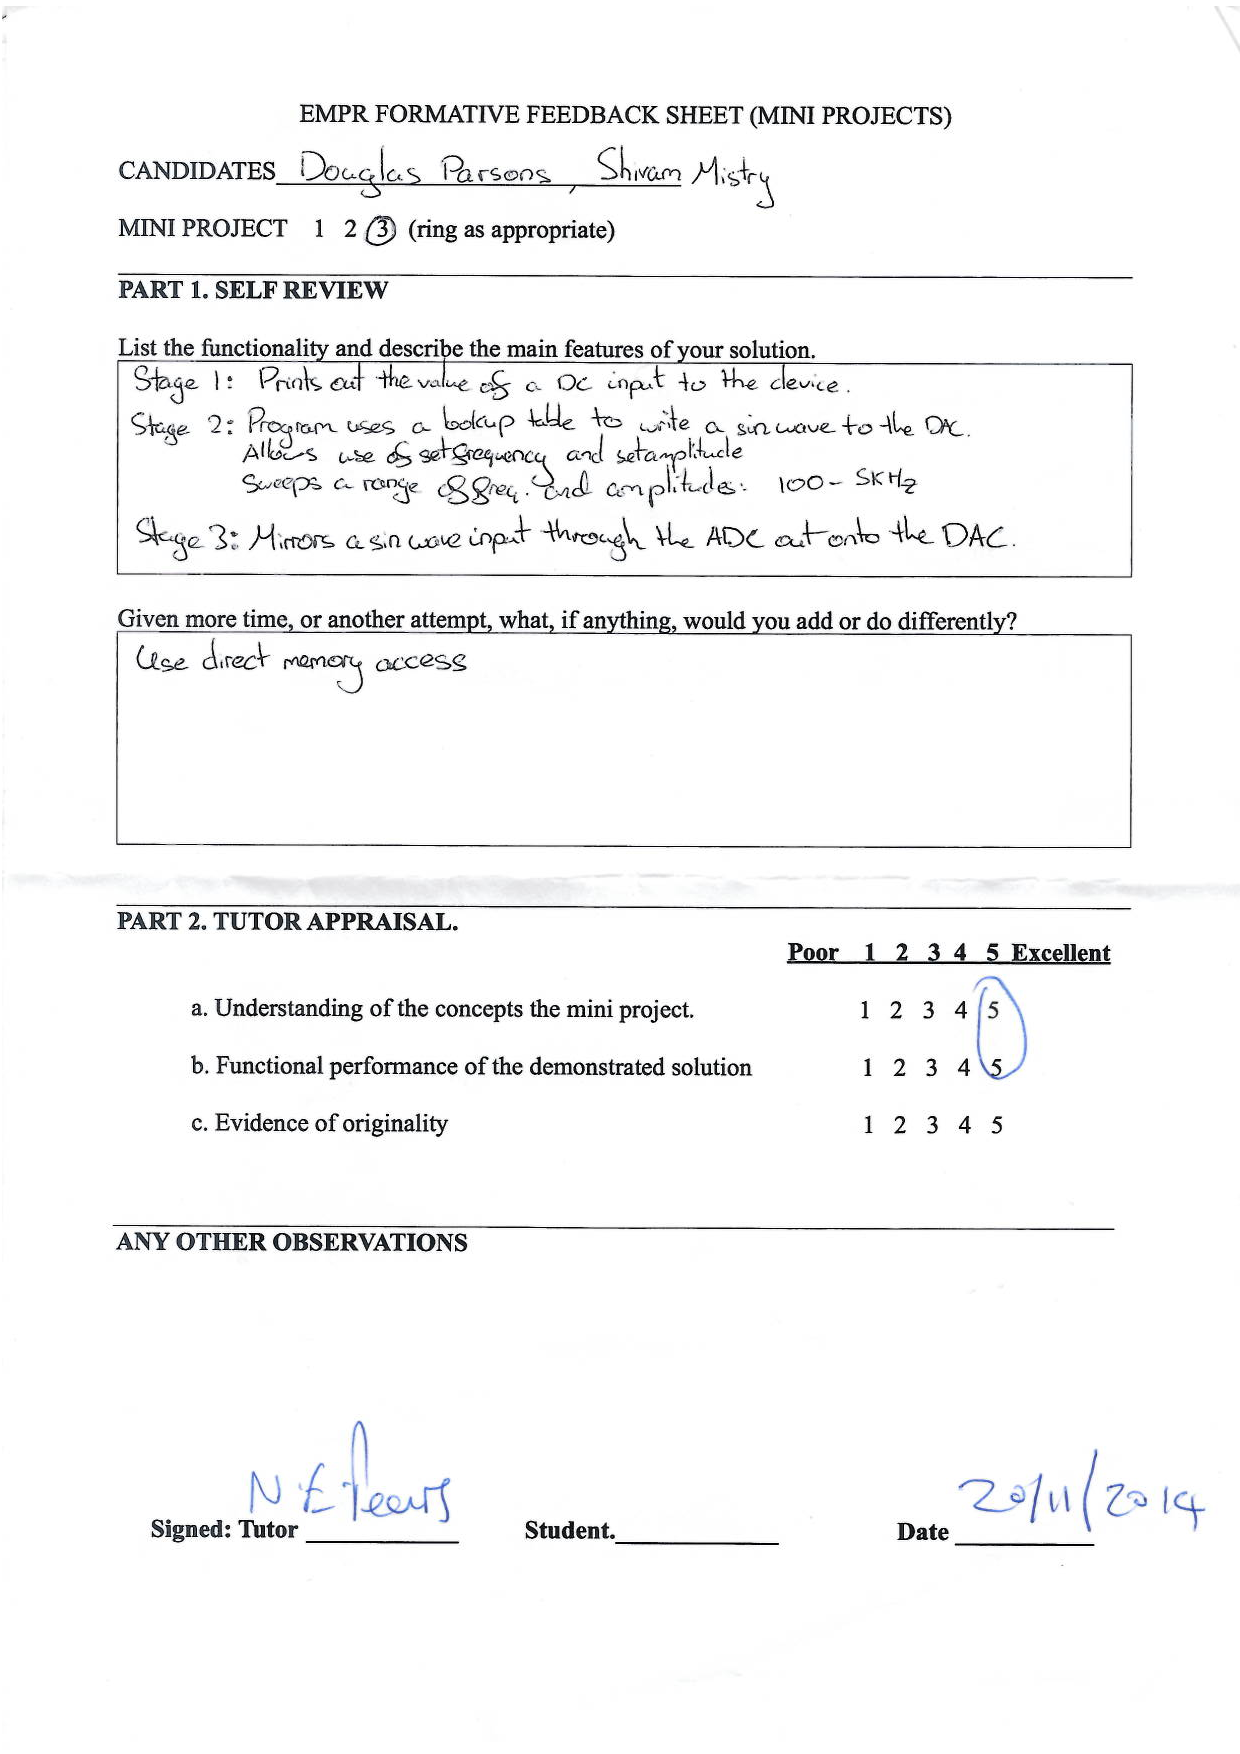
\includepdf[pages={1}]{mini_project_3.pdf}

\end{document}
